\documentclass{article}
\usepackage{graphicx} % Required for inserting images
\usepackage{tikz}
\usetikzlibrary{shapes.geometric, arrows}
\usepackage{hyperref}
\usepackage[backend=biber,style=authoryear]{biblatex}
\addbibresource{refs.bib}

\tikzstyle{box} = [rectangle, rounded corners, minimum width=3cm, minimum height=1cm, text centered, draw=black, fill=gray!30]
\tikzstyle{arrow} = [thick,->,>=stealth]

\title{Biology Classwork Investigation 15-8-2024}
\author{Sam K}
\date{August 2024}

\begin{document}

\maketitle

\section{Aim}
To justify the hierarchical structural organisation of organelles, cells, tissues, organ systems and organisms.

\section{Method}
\begin{enumerate}
    \item Use a number of sources to research the levels of organisation in multicellular organisms. Interactive  activities could be very useful in achieving the aim of this investigation. 
    \item When using a search engine, insert key words such as 'levels of organisation in multicellular organisms' + 'interactive' 
\end{enumerate}


\section{Flow Chart of Organisation From Least Complex to The Most Complex}
    \begin{center}
        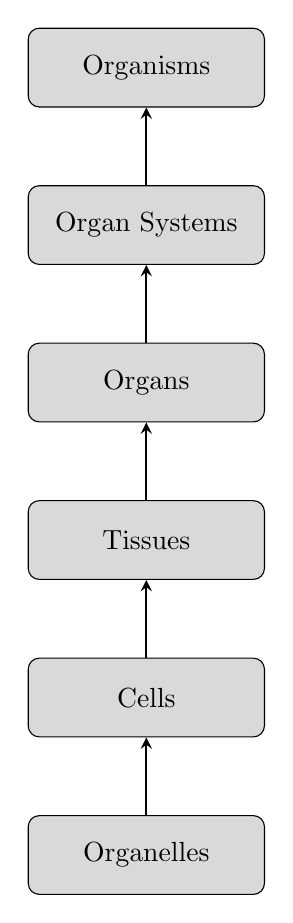
\begin{tikzpicture}[node distance=2cm]
    
        % Nodes
        \node (organelles) [box] {Organelles};
        \node (cells) [box, above of=organelles] {Cells};
        \node (tissues) [box, above of=cells] {Tissues};
        \node (organs) [box, above of=tissues] {Organs};
        \node (organSystems) [box, above of=organs] {Organ Systems};
        \node (organisms) [box, above of=organSystems] {Organisms};
        
        % Arrows
        \draw [arrow] (organelles) -- (cells);
        \draw [arrow] (cells) -- (tissues);
        \draw [arrow] (tissues) -- (organs);
        \draw [arrow] (organs) -- (organSystems);
        \draw [arrow] (organSystems) -- (organisms);
        
        \end{tikzpicture}
    \end{center}

\section{Class Functions}
\subsection{Organelles}
Organelles are specialized structures within a cell that perform distinct processes.

\textbf{Examples of Organelles}
\begin{itemize}
    \item \textbf{Nucleus} Contains genetic material (DNA) and controls cellular activities.
    \item \textbf{Mitochondria} Known as the powerhouse of the cell; they generate energy through cellular respiration.
    \item \textbf{Ribosomes} Synthesize proteins by translating genetic information from RNA.
    \item \textbf{Endoplasmic Reticulum (ER)}
    \begin{itemize}
        \item \textbf{Rough ER} Involved in protein synthesis and modification.
        \item \textbf{Smooth ER } Involved in lipid synthesis and detoxification.
    \end{itemize}
    \item \textbf{Golgi Apparatus} Modifies, sorts, and packages proteins and lipids for transport.
    \item \textbf{Lysosomes } Contain enzymes that break down waste materials and cellular debris.
    \item \textbf{Chloroplasts} Present in plant cells; responsible for photosynthesis.
    \cite{theeditorsofencyclopediabritanica_2023_structure}
\end{itemize}

By combining there specific functions of organelles, they work together to maintain the life, growth and reproduction of a cell

\subsection{Cells}
Cells are the basic structural and functional units of life. They are the smallest units that can carry out all life processes independently.

There are two kind of cells, \textit{prokaryotic}\footnote{"\textit{Pro}" : Without or false. \textit{"Karyotic"} : Nucleus} and \textit{eukaryotic}\footnote{"\textit{Eu}" : With or True. \textit{"Karyotic"} : Nucleus}

\textbf{Prokaryotic Cells}: These cells do not have a nucleus or other membrane-bound organelles. Example: Bacteria.
\textbf{Eukaryotic Cells}: These cells have a nucleus and other membrane-bound organelles. Example: Animal and plant cells.

Cells are responsible for carrying out various processes such as energy production (through cellular respiration), synthesis of molecules, and replication.
They contain DNA, the genetic material that controls cellular activities and passes on hereditary information. They are made up of a plasma membrane, cytoplasm, and various organelles, each performing specific functions. \cite{stavans_1993_the}

\subsection{Tissues}
Tissues are groups of similar cells that work together to perform a specific function.

Tissues work together to form organs, contributing to more complex functions.
They provide structure and support to the body, enable movement, and facilitate communication between different parts of the body.

\textbf{Types of Tissues}
\begin{itemize}
    \item \textbf{Epithelial Tissue} Covers body surfaces and lines body cavities. Example: Skin \& lining of the stomach.
    \item \textbf{Connective Tissue} Supports, binds, and protects other tissues and organs. Example: Bone, blood, cartilage.
    \item \textbf{Muscle Tissue} Responsible for movement. Example: Skeletal muscles, heart muscles.
    \item \textbf{Nervous Tissue} Transmits nerve impulses throughout the body. Example: Brain \& spinal cord.
    \cite{overholtzer_2008_the}
\end{itemize}

\subsection{Organs}
Organs are structures composed of two or more different types of tissues that work together to perform a specific function.

Organs are vital for the survival and functioning of an organism.
Each organ has a unique role, contributing to the body's homeostasis and overall health.

\textbf{Examples of Organs}
\begin{itemize}
    \item \textbf{Heart} Pumps blood throughout the body.
    \item \textbf{Lungs} Facilitate the exchange of oxygen and carbon dioxide.
    \item \textbf{Liver} Processes nutrients and detoxifies harmful substances.
    \item \textbf{Kidneys} Filter blood and produce urine.
    \item \textbf{Stomach} Digests food and absorbs nutrients.
    \cite{a2016_europe}
\end{itemize}

\subsection{Organ Systems}

\subsection{Organisms}
Organisms are individual living entities that can carry out all basic life processes independently.

Organisms exhibit the characteristics of life, including growth, reproduction, response to stimuli, and metabolism.
They interact with their environment, obtain energy, and maintain homeostasis.

\textbf{Types of Organisms}
\begin{itemize}
    \item \textbf{Single-celled Organisms:} Composed of only one cell. Example: Bacteria \& amoebas.
    \item \textbf{Multicellular Organisms:} Composed of multiple cells organized into tissues, organs, and organ systems. Example: Humans, plants \& animals.
\end{itemize}

In multicellular organisms, cells, tissues, organs, and organ systems work together in a highly organized manner to ensure survival and reproduction. \cite{a2016_europe}

\section{Relationship of Levels of Organisation}

\begin{center}
    \includegraphics[scale=0.2]{holatex.png}
\end{center}

\newpage
\printbibliography

\end{document}
